\documentclass[a4paper,11pt,fleqn]{article}%fleqn pour aligner les equations à gauche
\usepackage{../../Styles/Cours}


\newcommand{\chnum}{Chapitre 19}
\newcommand{\chtitle}{Lunette astronomique}
\newcommand{\dtype}{Cours}
  
\begin{document}
	\maketitle
	
	\section{Description}
		\subsection{Usage}
		La lunette astronomique est un instrument optique permettant d'observer des objets lointains en grossissant leur taille apparente. Inventée à la fin du {16}$^e$ siècle, elle a permis par exemple à Galilée de découvrir quelques années plus tard les reliefs de la Lune et les satellites de Jupiter ou encore d'observer que la Voie Lactée était faite d'étoiles.
		
		\subsection{Constitution}
		Une lunette astronomique est composée de deux systèmes optiques convergents. Elle peut être modélisée par un système de deux lentilles convergentes ayant un axe optique commun :
		\begin{itemize*}
			\item l'\textbf{objectif} situé du côté de l'objet observé
			\item l'\textbf{oculaire} du côté de l'\oe il.
		\end{itemize*}
		La distance focale de l'objectif est supérieure à la distance focale de l'oculaire.\\
		Lorsque le foyer image $F'_1$ de l'objectif et le foyer objet $F_2$ de l'oculaire sont confondus, la lunette est dite \textbf{afocale}.
		\begin{center}
			\begin{tikzpicture}[scale=.72,transform shape]
				\draw[dashed,line width=1.2pt](-6,0) -- (10,0);
				\draw[Latex-Latex] (0,-2) to (0,2);
				\draw[Latex-Latex] (6.25,-2) to (6.25,2);
				\draw (5,0) node {\Large $|$} ;
				
				
				\draw (0,0) node[below left]{\Large $O_1$};
				\draw (6.25,0) node[below right]{\Large $O_2$};
				\draw (5,0.1) node[above]{\Large $F_1'$ $et$ $F_2$};
				
				\draw (0,2) node[above]{\textbf{\Large Objectif}};
				\draw (6.25,2) node[above]{\textbf{\Large Oculaire}};
				
				\draw (-5,-0.2) node[below]{\Large $F_1$};
				\draw (-5,0) node {\Large $|$} ;
				\draw (7.5,0.1) node[above]{\Large $F'_2$};
				\draw (7.5,0) node {\Large $|$} ;
				\draw (10,0.1) node[above]{\Large $\Delta$};
			\end{tikzpicture}
		\end{center}
		
	\section{Image à travers une lunette astronomique}
		\subsection{Objet à l'infini}
	\noindent\begin{minipage}{\linewidth}
			Pour construire l'image d'un objet $AB$ à travers une lentille, on trace différents rayons lumineux issus du point $B$ de l'objet.\\
			Lorsque cet \textbf{objet} est \textbf{infiniment éloigné}, on considère que les rayons lumineux qui sont issus du point $B$ sont parallèles entre eux. (cas n° 3 de l'image ci-contre)
		\end{minipage}
	\begin{minipage}{\linewidth}
		\begin{center}
			\begin{tikzpicture}[scale=.5,transform shape]
				\draw[line width=1.2pt](-6,0) -- (1,0);
				\draw[Latex-Latex] (0,-2) to (0,2);
				\draw (-1,2) node{\huge B};
				\draw[-Latex,red!80!black,line width=1.2pt](-1,1.5) to (0,2); 
				\draw[-Latex,red!80!black,line width=1.2pt](-1,1.5) to (0,0);  
				\draw[-Latex,red!80!black,line width=1.2pt](-1,1.5) to (0,-2);
		\end{tikzpicture} \hspace{1cm}
	\begin{tikzpicture}[scale=.5,transform shape]
		\draw[line width=1.2pt](-6,0) -- (1,0);
		\draw[Latex-Latex] (0,-2) to (0,2);
		\draw (-6,2) node{\huge B};
		\draw[-Latex,red!80!black,line width=1.2pt](-6,1.5) to (0,2); 
		\draw[-Latex,red!80!black,line width=1.2pt](-6,1.5) to (0,0);  
		\draw[-Latex,red!80!black,line width=1.2pt](-6,1.5) to (0,-2);
	\end{tikzpicture}\hspace{1cm}
	\begin{tikzpicture}[scale=.5,transform shape]
		\draw[line width=1.2pt](-6,0) -- (1,0);
		\draw[Latex-Latex] (0,-2) to (0,2);
		\draw (-6,0) node[above]{\huge B$_{\infty}$};
		\draw[-Latex,red!80!black,line width=1.2pt](-6,2) to (0,2); 
		\draw[-Latex,red!80!black,line width=1.2pt](-6,0) to (0,0);  
		\draw[-Latex,red!80!black,line width=1.2pt](-6,-2) to (0,-2);
	\end{tikzpicture}
			
		\end{center}
	\end{minipage}
		
		
		\subsection{Image à travers l'objectif}
		On considère un objet $AB$ situé "à l'infini".
		\begin{enumerate}
			\item Tracer le rayon issu de $B$ passant par le centre optique $O_1$, il n'est pas dévié.
			\item Tracer le rayon issu de $B$ passant par le foyer objet $F_1$, il émerge parallèlement à l'axe optique.
		\end{enumerate}
		Les deux rayons se croisent au  point $B_1$, image du point $B$ à travers l'objectif. Il se situe dans le \textbf{plan focal image} de l'objectif.\\
		L'image $A_1B_1$ de l'objet $AB$ à travers l'objectif est réelle et renversée par rapport à l'objet. Elle devient objet pour la deuxième lentille (l'oculaire), c'est pourquoi on parle d'\textbf{image intermédiaire}.
		
		\subsection{Image à travers l'oculaire}
		L'image intermédiaire $A_1B_1$ sert d'objet pour l'oculaire.
		\begin{enumerate}[resume]
			\item Prolonger tous les rayons précédents jusqu'à l'oculaire.
			\item Poursuivre le rayon 2, il est parallèle à l'axe optique et émerge de l'oculaire en passant par le foyer image $F'_2$.
			\item Tracer le rayon issu de $B_1$ passant par le centre optique $O_2$, il n'est pas dévié.
		\end{enumerate}
		Les deux rayons ne se croisent pas, ils émergent de l'oculaire en étant parallèles entre eux. Ce sera donc le cas pour tous les rayons émergeant de l'oculaire. L'\textbf{image définitive $\mathbf{A_2B_2}$} se situe donc \textbf{"à l'infini"}.
		\begin{enumerate}[resume]
			\item Poursuivre le rayon 1, il émerge de l'oculaire parallèlement aux deux rayons précédents.
		\end{enumerate}
		\begin{center}
		\begin{tikzpicture}[scale=.9,transform shape,>=stealth']
			\tikzset{fleche/.style args={#1:#2}{ postaction = decorate,decoration={name=markings,mark=at position #1 with {\arrow[#2,scale=2]{>}}}}}
			
			\foreach \k in {-7,-6.5,...,13.5} {\draw[gray!30] (\k,-4) -- (\k,4);}
			\foreach \k in {-4,-3.5,...,4} {\draw[gray!30] (-7,\k) -- (13.5,\k);}
			\draw[dashed,line width=1.2pt](-6.5,0) -- (13,0);
			\draw[Latex-Latex] (0,-3) to (0,3);
			\draw[Latex-Latex] (6.5,-3) to (6.5,3);
			%\draw (5,0) node {\Large $|$} ;
			
			
			\draw (0,0) node[below left]{\Large $O_1$};
			\draw (6.5,0) node[below right]{\Large $O_2$};
			\draw (4.5,1.5) node{\Large $F_1'$ $et$ $F_2$};
			\draw[dashed,line width=1.2pt] (4.5,-3)--(4.5,3);
			
			\draw (0,3) node[above]{\textbf{\Large Objectif}};
			\draw (6.5,3) node[above]{\textbf{\Large Oculaire}};
			
			\draw (-4.5,-0.5) node[below]{\Large $F_1$};
			\draw (-4.5,0) node {\Large $|$} ;
			\draw (8.5,-0.5) node[below]{\Large $F'_2$};
			\draw (8.5,0) node {\Large $|$} ;
			\draw (12,0.1) node[above]{\Large $\Delta$};
			
			\draw[fleche=0.5:blue,blue] (-6,2)to(0,0);
			\draw[blue] (-6,2) node[left]{\Large B$_{\infty}$};
			\draw[blue] (-6.5,0) node[above]{\Large A$_{\infty}$};
			\end{tikzpicture}
	\end{center}
	
		\subsection{Bilan}
		Des rayons arrivant que une lunette afocale parallèles entre eux en ressortent également parallèles entre eux. L'image d'un objet "à l'infini" se situe donc elle-même "à l'infini". Cela caractérise un système \textbf{afocal}.\\
		Intérêt : l'image définitive étant située "à l'infini", il est possible de l'observer dans effort (l'\oe il reste au repos car il n'a pas besoin de s'accommoder).
		
	\section{Données commerciales}
		\subsection{Grossissement}
		La \textbf{taille apparente} d'un objet est l'angle sous lequel les extrémités de l'objet sont observés.\\
		\textcolor{gray!80}{Exemple : Depuis la Terre, la Lune et le Soleil ont une taille apparente similaire. Lorsque la Lune passe devant le Soleil, cela donne lieu à des éclipses de Soleil spectaculaire. De tels éclipses seraient impossibles si la Lune avait une taille apparente inférieure au Soleil.}\\
		
	\noindent \begin{minipage}{.6\linewidth}
			L'image d'un objet à travers une lunette astronomique afocale est vue sous un \textbf{angle} $\theta '$ supérieur à l'angle $\theta$ sous lequel l'objet est vu à l'\oe il nu. Le rapport entre les deux angles est appelé \textbf{grossissement} :\\
			\begin{tabular}{c|m{6.5cm}}
				\multirow{3}{4cm}{\centering $G = \dfrac{\theta '}{\theta}$} & $\theta '$ : angle sous lequel est vue l'image à travers la lunette afocale\\
				& $\theta '$ : angle sous lequel est vue l'objet à l'\oe il nu\\
				& Les angles doivent être exprimés dans la même unité.
			\end{tabular}\\
		\end{minipage}
	\begin{minipage}{.4\linewidth}
		\centering 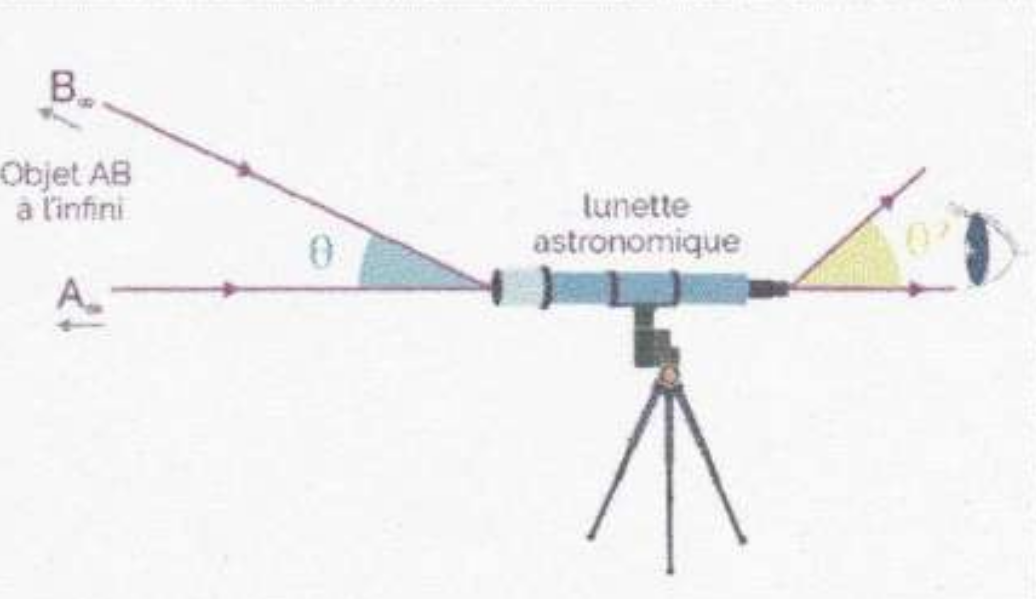
\includegraphics[width=\linewidth]{Ressources/TSPE_C13_Cours_Fig1.png}
	\end{minipage}
	
	\textbf{Attention !} Ne pas confondre le \emph{grossissement} $G$ qui est le rapport d'angle et le \emph{grandissement} $\gamma$ qui est un rapport de longueur !\\
	Le grossissement peut être exprimé en fonction des distances focales des deux lentilles. le raisonnement est le suivant (\textbf{à connaître}) :\\
	\fbox{\begin{minipage}{\linewidth}
			Pour des angles suffisamment petits, on peut faire l'approximation $\theta \approx\tan{\theta}$. C'est le cas ici car les objets observés sont lointains. Ainsi $\theta \approx \tan{\theta}$ et $\theta ' \approx \tan{\theta '}$\\
			
			Or, d'après le schéma : $\tan{\theta}=\dfrac{A_1B_1}{O_1A_1} = \dfrac{A_1B_1}{f'_1}$ et  $\tan{\theta'}=\dfrac{A_1B_1}{A_1O_2} = \dfrac{A_1B_1}{f'_2}$\\
			Donc :
			\begin{equation}
				G = \frac{\theta '}{\theta}=\dfrac{\tan{\theta'}}{\tan{\theta}} = \dfrac{\dfrac{A_1B_1}{f'_2}}{\dfrac{A_1B_1}{f'_1}} = \dfrac{A_1B_1}{f'_2} \times \dfrac{f'_1}{A_1B_1}  = \dfrac{f'_1}{f'_2} \nonumber
			\end{equation}
		Le grossissement d'une lunette afocale s'écrit donc :\\
		\begin{tabular}{c|l}
			\multirow{3}{4cm}{\centering $G = \dfrac{f'_1}{f'_2}$} & $f'_1$ : distance focale de l'objectif (en \unit{\meter})\\
			& $f'_2$ : distance focale de l'oculaire (en \unit{\meter})\\
		\end{tabular}
	\vspace{.5cm}
	
	\end{minipage}}
		
		\subsection{Luminosité}
		\noindent \begin{minipage}{.6\linewidth}
			Les faisceaux lumineux collectés par la lumière sont limités par la taille de l'objectif. plus le \textbf{diamètre de l'objet} est grand, plus la quantité de lumière collectée par la lunette et pénétrant ensuite dans l'\oe il à la sortie de l'oculaire est grand.\\
			Une lunette astronomique est donc caractérisée par le \textbf{diamètre et la distance focale de son objectif}, exprimés en millimètre.
		\end{minipage}
	\begin{minipage}{.4\linewidth}
		\centering 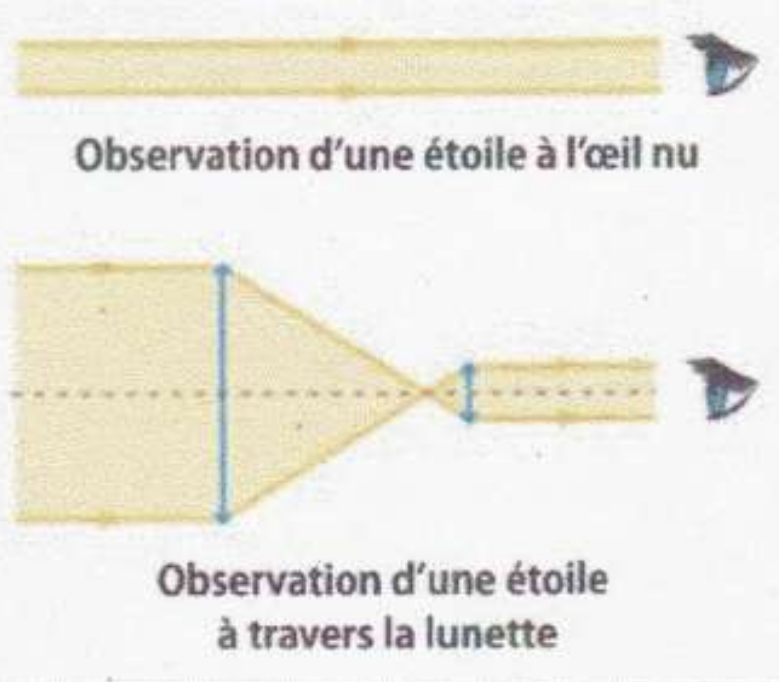
\includegraphics[width=\linewidth]{Ressources/TSPE_C13_Cours_Fig2.png}
	\end{minipage}
\end{document}